%TODO Why is the global status relevant
%Is there other things that should be described in the report

\section{State Machine}
The watchdog manager has a state machine, shown in
figure~\ref{FIG:GLOBALSTATUSES}. Its transitions depend on the changes of the
global variables, and the current state. If the behavior of the watchdog manager
is correct and the manager is activated, it will stay in the state
'WDGM\_GLOBAL\_STATUS\_OK'. There are however lots of reasons for that the
status will change from the correct state. It depends on the arguments of the
API calls but also the order of the commands that are called and which AUTOSAR
configuration that is supplied. The configuration is important because it
specifies the tolerance of faulty behavior the watchdog should have. It could
also indirectly disable some states and state transition or make some
transition more likely to happen. The effect can for instance come from the
number of checkpoints supplied in the configuration. A correct behavior of the
watchdog manager depends on that checkpoints are reached with correct timing
and does so in the right order.

Besides the transition between the deactivated and the OK states, the only
function that can give rise to state transitions for the global status, is the
main function. In an working ECU, the main function should continuously be
called, in a configured time interval, by the run time environment (RTE). Note
that the timing is not used when using QuickCheck, see section
\ref{SEC:CALLING_COMMANDS}.

\begin{figure}[h!]
  \begin{center}
    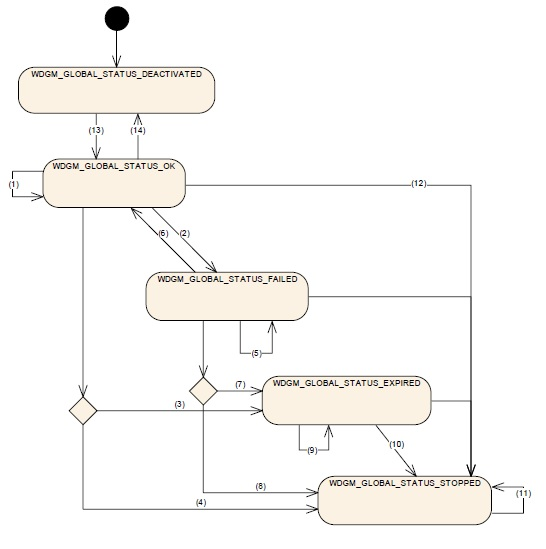
\includegraphics{pictures/globalstatuses.jpg}
  \end{center}
  \caption{State diagram that shows possible trasitions between states}
  \label{FIG:GLOBALSTATUSES}
\end{figure}

\section{Configurations}
The WdgM was tested using three different configurations. The configurations
were of different complexity. One was a minimal configuration, one a example
configuration and one was a live configuration, used in actual implementations.

Because there is only a small number of commands that influences the state
transitions, those commands were tweaked and therefore was generated more
often. On the other hand, all get-functions were tweaked to not be generated as often.

\subsection{BSI}
A highly simplified configuration, \emph{BSI}, gives in some sense good results.
Using this configuration the WdgM was never hitting the absorbing state
according to figure \ref{FIG:GLOBALSTATUSES}.  However looking at the state
transitions, comparing figure \ref{FIG:GLOBALSTATUSES} and table
\ref{TABLE:STATUSES_BSI}, only two states are hit. This happens
because the configuration is to simple, it is actually impossible to hit
any other states then \emph{'GLOBAL\_STATUS\_OK'} or
\emph{'GLOBAL\_STATUS\_DEACTIVATED'}. There are no checkpoints or supervision
functions configured for the \emph{BSI} configuration.
It is easy to run tests using this configuration but it does not, by it self,
fully test the code because some specification requirements will never be
tested. The untested requirements are mainly requirements for supervision
functions that are, according to the configuration, never supposed to be
run. Those untested requirements leaves also other requirements untested because
the watchdog manager never reaches a state when those other requirements must
hold.

Figure~\ref{FIG:COMMANDS_BSI} shows how many times a certain command was
generated versus the length of the command sequence that was generated. E.g. the
function \lstinline!WdgM_CheckpointReached! had in average a little more than
40\% of all calls. This is because, in any other configuration, the supervision
functions demand that a certain number of checkpoints is reached before the next
main function is called \footnote{This is however not completely true, but it
  gives the general idea.}. There is also a dependency the other way around. The
main function has to be called a certain number of times before
\lstinline!WdgM_CheckpointReached! is called on a certain supervised
entity. This is why that function also has quite high proportions. Other
functions that stands out is \lstinline!WdgM_SetMode! and \lstinline!WdgM_Init!.
\lstinline!WdgM_Setmode! is called because different modes can have different
supervision functions and supervised entities. That is why we need to call this
function often. It should retain the states of supervised entities that is
activated in the new mode and should reset the local state if the entity is
deactivated in the new mode. The function \lstinline!WdgM_Init! is in contrast
called lesser and lesser times. This function is only needed when the global
state is deactivated. It has more likelihood to be generated among the first
commands in the command sequence, or right after a \lstinline!WdgM_DeInit!.

\begin{figure}[!ht]
  \begin{center}
    \subfigure[Shows percentage of each possible command executed]{
      \label{FIG:COMMANDS_BSI}
      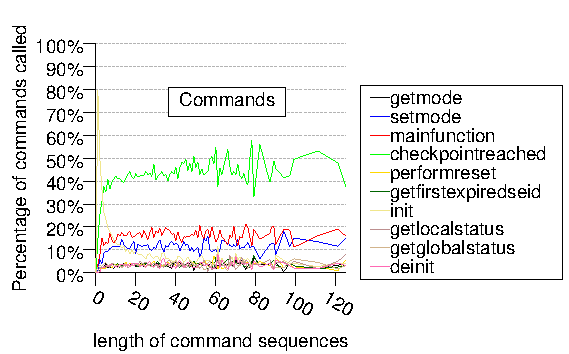
\includegraphics{generated_pictures/history_commands_bsi.pdf}
    }

    \subfigure[Shows percentage of each possible global status hit]{
      \label{FIG:STATUSES_BSI}
      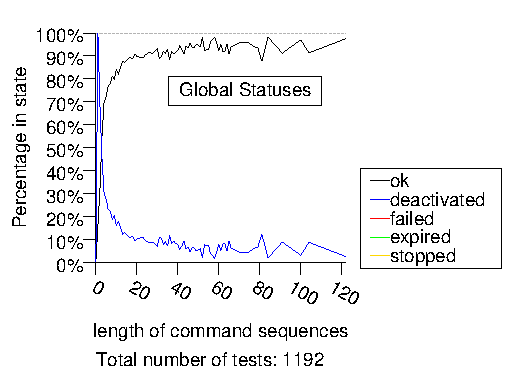
\includegraphics{generated_pictures/history_statuses_bsi.pdf}
    }
  \end{center}
  \caption{BSI configuration}
  \label{FIG:BSI}
\end{figure}

\begin{table}[!ht]
  \caption{BSI configuration}
  \label{TABLE:STATUSES_BSI}
  
    \begin{tabular}{r|ccccc}
        \hline
        \multicolumn{6}{c}{Number of tests: 2850} \\
        \hline
        \backslashbox{From}{To}
                    & DEACTIVATED & EXPIRED & FAILED & OK & STOPPED \\
        \hline
        DEACTIVATED & \bf{02.23}\% & 00.00\%       & 00.00\%       & \bf{09.12}\% & 00.00\% \\
        EXPIRED     & 00.00\%       & \bf{00.00}\% & 00.00\%       & 00.00\%       & \bf{00.00}\% \\
        FAILED      & 00.00\%       & \bf{00.00}\% & \bf{00.00}\% & \bf{00.00}\% & \bf{00.00}\% \\
        OK          & \bf{03.24}\% & \bf{00.00}\% & \bf{00.00}\% & \bf{85.41}\% & \bf{00.00}\% \\
        STOPPED     & 00.00\%       & 00.00\%       & 00.00\%       & 00.00\%       & \bf{00.00}\%
      \end{tabular}
    

\end{table}

\subsection{Freescale}
The Freescale configuration is, compared to BSI, a more realistic configuration.
All supervision algorithms are configured and there are both external and
internal graphs for logical supervision. It is also one of the configurations
that is used in actual lab environments. The state machine for the global
status is totally covered by running QuickCheck, see
table~\ref{TABLE:STATUSES_FREESCALE} and figure~\ref{FIG:GLOBALSTATUSES}.

\begin{figure}[!ht]
  \begin{center}
    \subfigure[Shows percentage of each possible command executed]{
      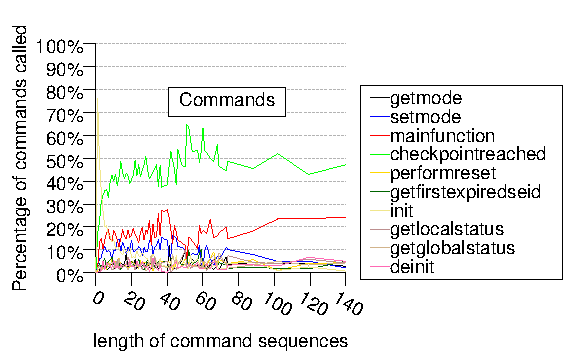
\includegraphics{generated_pictures/history_commands_freescale.pdf}
      \label{FIG:COMMANDS_FREESCALE}
    }
    \subfigure[Shows percentage of each possible global status hit]{
      \label{FIG:STATUSES_FREESCALE}
      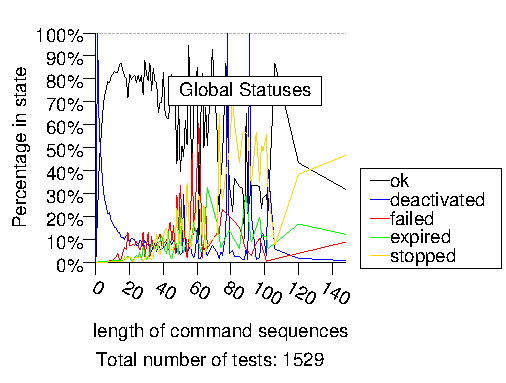
\includegraphics{generated_pictures/history_statuses_freescale.pdf}
    }
  \end{center}
  \caption{Freescale configuration}
  \label{FIG:FREESCALE}
\end{figure}

\begin{table}[!ht]
  \caption{Freescale configuration}
  \label{TABLE:STATUSES_FREESCALE}
  
    \begin{tabular}{r|ccccc}
        \hline
        \multicolumn{6}{c}{Number of tests: 1023} \\
        \hline
        \backslashbox{From}{To}
                    & DEACTIVATED & EXPIRED & FAILED & OK & STOPPED \\
        \hline
        DEACTIVATED & \bf{02.43}\% & 00.00\%       & 00.00\%       & \bf{08.32}\% & 00.00\% \\
        EXPIRED     & 00.00\%       & \bf{03.36}\% & 00.00\%       & 00.00\%       & \bf{00.11}\% \\
        FAILED      & 00.00\%       & \bf{00.17}\% & \bf{07.77}\% & \bf{00.12}\% & \bf{00.11}\% \\
        OK          & \bf{02.56}\% & \bf{00.18}\% & \bf{00.87}\% & \bf{69.53}\% & \bf{00.12}\% \\
        STOPPED     & 00.00\%       & 00.00\%       & 00.00\%       & 00.00\%       & \bf{04.34}\%
      \end{tabular}
    

\end{table}

\subsection{Example}
The example configuration is somewhat more complex than the Freescale
configuration. This is because it supports all functionality of an
configuration. Because of the complexity, some transition is harder or even
impossible to reach. Noticeable is that the transition from the failed to
the okay state, according to figure \ref{FIG:GLOBALSTATUSES} is never made, see
table \ref{TABLE:STATUSES_EXAMPLE}. The reason for that is that the alive
functions must fail once and then continue without failures. Because
\lstinline!WdgM_MainFunction! handles the alive supervision calculations, and
the function \lstinline!WdgM_CheckpointReached! handles the incrementation of
the alive counters. A certain number of calls to
\lstinline!WdgM_CheckpointReached! must be done between each
\lstinline!WdgM_MainFunction!. It does not stop there. Each checkpoint may have
some logical supervision, so the order of the called checkpoints is important as
well. It is also possible to set deadline supervision for a supervised
entity. Both deadline supervision and logical supervision is handled by
\lstinline!WdgM_CheckpointReached!, but with deadline supervision some time,
specified in the configuration, must have elapsed since the start
checkpoint. Because ``time'' isn't specified in AUTOSAR, see
section~\ref{SEC:FUNCTIONAL_SAFETY_TIME}, the model implemented time as the
c-code, with the use of \lstinline!WdgM_MainFunction!. This is possible because
we know that \lstinline!WdgM_MainFunction! is called periodically.
% We tried hard to find a suitable example when the global status transited from
% \lstinline!WDGM_GLOBAL_STATUS_FAILED! to \lstinline!WDGM_GLOBAL_STATUS_OK!, in
% the example configuration, but the number of commands needed for this
% transition expanded to much and somewhere some other supervision failed.

\begin{figure}[!ht]
  \begin{center}
    \subfigure[Shows percentage of each possible command executed]{
      \label{FIG:COMMANDS_EXAMPLE}
      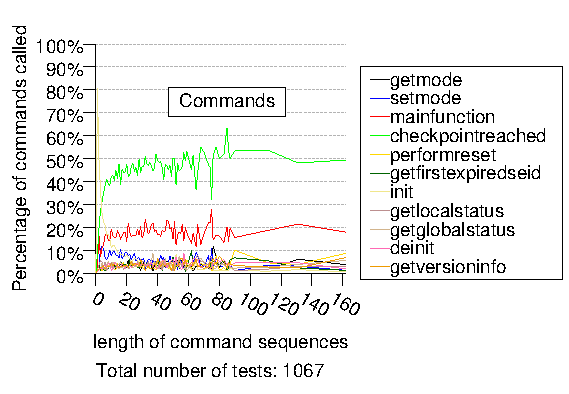
\includegraphics{generated_pictures/history_commands_example.pdf}
    }

    \subfigure[Shows percentage of each possible global status hit]{
      \label{FIG:STATUSES_EXAMPLE}
      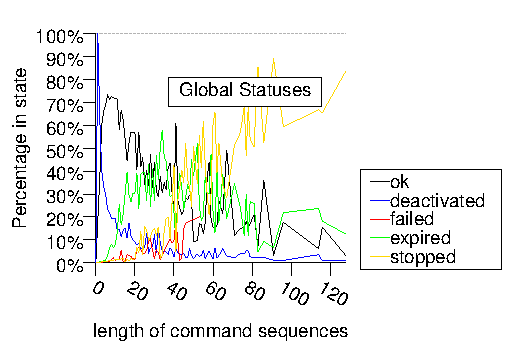
\includegraphics{generated_pictures/history_statuses_example.pdf}
    }
  \end{center}
  \caption{Example configuration}
  \label{FIG:EXAMPLE}
\end{figure}

\begin{table}[!ht]
  \caption{Example configuration}
  \label{TABLE:STATUSES_EXAMPLE}
  
    \begin{tabular}{r|ccccc}
        \hline
        \multicolumn{6}{c}{Number of tests: 3877} \\
        \hline
        \backslashbox{From}{To}
                    & DEACTIVATED & EXPIRED & FAILED & OK & STOPPED \\
        \hline
        DEACTIVATED & \bf{02.59}\% & 00.00\%       & 00.00\%       & \bf{07.81}\% & 00.00\% \\
        EXPIRED     & 00.00\%       & \bf{24.77}\% & 00.00\%       & 00.00\%       & \bf{00.81}\% \\
        FAILED      & 00.00\%       & \bf{00.12}\% & \bf{02.87}\% & \bf{00.00}\% & \bf{00.04}\% \\
        OK          & \bf{01.68}\% & \bf{02.50}\% & \bf{00.39}\% & \bf{40.22}\% & \bf{00.14}\% \\
        STOPPED     & 00.00\%       & 00.00\%       & 00.00\%       & 00.00\%       & \bf{16.07}\%
      \end{tabular}
    

\end{table}

\section{Handle bugs in the C code}
\label{sec:handlebugs}
There is a number of possible ways to handle bugs when QuickCheck encounters
them. The problem is that QuickCheck generates arbitrary command sequences, it
cannot ``save'' an error and proceed to find the next error. Either the c-code
or the model needs to be ``corrected''.
The best way, with the model in mind, would often be to let a third
party correct the discovered bugs. However this is time consuming because the
support line has often already much to do, and the releases doesn't come that
often.
Another way is to mock the erroneous function, but then you will only find one
bug per function, strictly limiting the probability to find bugs.
Then there is two equally good methods. Either the Erlang model needs to have
the fault implemented, or the c-code needs to be fixed. There are pros and cons
with both methods. If the Erlang model introduce bugs, there may be secondary
failures which are not discovered. This could also happened when correcting the
c-code, but then more knowledge of the module is needed, and some of the
secondary failures can easier be avoided. It also takes more time to get the
extra knowledge of the c-code.

We choose to correct the c-code, because then we had direct feedback and could
discover where in the code the bugs were introduced.

\section{Functional safety analysis}
\subsection{Definition of time}
\label{SEC:FUNCTIONAL_SAFETY_TIME}
Because of ambiguities in AUTOSAR, time isn't defined, but it is still needed
for deadline supervision. In deadline supervision when a start checkpoint is
reached, a timer should start. If the final checkpoint is not reached within a
configured time marginal, then the deadline supervision for the supervised
entity with the given checkpoint will fail.
The problem is as mentioned the definition of time. Because we know that
\lstinline!WdgM_MainFunction! should be called periodically, it could be used
for the measurements of time. For each call of \lstinline!WdgM_MainFunction!
tick a ``time'' counter.

\section{Statistics}
The distribution of API-calls seems, according to figure
\ref{FIG:COMMANDS_BSI}, \ref{FIG:COMMANDS_FREESCALE} and
\ref{FIG:COMMANDS_EXAMPLE}, to be the same for all configuration. The arguments
to the API calls is however different, even though it is not seen in those plots.
The most interesting API calls is the ones thats modifies the internal state of
the wathdog mangager, see appendix \ref{APP:API_CALLS}, namely \emph{init},
\emph{deinit}, \emph{setmode}, \emph{mainfunction},
\emph{checkpointreached} and \emph{performreset}. The reason for this is that
they will influence the results of future coming API calls.

The init and deinit functions can just put the global
status between two states, and should only change the internal state of the
watchdog, when the watchdog is in either \emph{WDGM\_GLOBAL\_STATUS\_OK}
or \emph{WDGM\_GLOBAL\_STATUS\_DEACTIVATED}, according to
figure \ref{FIG:GLOBALSTATUSES}. If this happens they will change the internal
state of the watchdog but will do so in the same manner independent previous
called commands. The behaviour of this commands will hence not vary much.
This two functions has also the property that after they are called they will
always put the watchdog manager in the same state, or a state that has already
been reached, except for the first time the init function is called.

The performreset function is boring why?

The set mode function changes the mode, why interesting?

The two remaining API-calls that are really worth discussing in detailed are the
main function and the checkpoint reached function. As can be seen in
\ref{FIG:COMMANDS_BSI}, \ref{FIG:COMMANDS_FREESCALE} and \ref{FIG:COMMANDS_EXAMPLE},
\ref{FIG:COMMANDS_EXAMPLE} they are also the two commands that are most most
often called.

\section{Coverage}
\subsection{Erlang module}
The Erlang module \emph{cover} was used to calculate the code coverage for the
Erlang module. The line coverage results was ??.
\subsection{C-code}
Bullseye Coverage was used to analyse the coverage of the C-code. The results
show that the decision coverage is over ?? and all functions except for one is
covered, see figure \ref{FIG:BULLSEYE}. The reason, for that there is a function
that is not covered, is that it is deprecated and hence not implemented in Erlang
code. Missing decision coverage in the C-code are checks for null pointers,
which never evaluated to false. Many such checks seems to be redundant and
impossible to evaluate to true, if one
excludes the possibility of hardware failures or other processes which may
corrupt the memory of the watchdog manager.

The coverage statistics shown in \ref{FIG:BULLSEYE} is constructed
using three configuration. Using several configuration gave better results since
some code is impossible to reach if not certain configuration parameters are set.

\begin{figure}[!ht]
\caption{Shows coverage statistics generated by Bullseye Coverage}
\label{FIG:BULLSEYE}
\end{figure}


\section{Functional safety analysis}
Since one important part of the functional safety concept is that it must be
taken in consideration during the hole development process, one can not simply
say that QuickCheck makes it possible to acquire functional safety. There must
first be a number of assumptions. Not even if it is assumed that
every step in the development, until the actual implementation of the watchdog
manager, satisfies the requirements one also has to assume that the remaining
part of the development, towards a finished vehicle, follows the same
constrains. Even further, if this is assumed, there is one important
assumption left before
one can even reason about how QuickCheck can benefit.
This assumptions lies in that the model for the watchdog
manager is correct, namely the AUTOSAR specification.


%% LoC
%% right side of pipe:  without blank lines and comments
%% *.c files: 3271 | 1736
%% *.h files: 18964 | 10942
%% total c-code: 22235 | 12678
%% *.erl: 2006 | 1470
%% *.hrl: 68 | 64
%% total erlang: 2074 | 1534
